%*****************************************************
%	APPENDIX
%*****************************************************
\chapter{Ocean Wave Derivations}
\label{ap:oceanWaves}

\section{Random Phase/Amplitude Model} \label{sec:ap.oceanWaves.randModel}

Initially considering a \gls{waveRecord}, this \gls{waveRecord} can be reconstructed using a Fourier series with $a_{i}$ and $\phi_{i}$ represent the amplitude and phase. The underscore on each variable represents a random variable.

\begin{equation} \label{eq:ap.waveSpectrum.fourierSeries}
    \underline{\eta}(t) = \sum_{i=1}^{N}\underline{a}_{i}cos(2\pi f_{i}t + \underline{\phi}_{i})
\end{equation}

Where $f_{i}=i/D$, which gives rise to a frequency interval, $\Delta f=1/D$. Fourier analysis allows an amplitude and frequency spectrum to be determined.
(Could include image of pg. 32 [Fig. 3.4] OR pg.34)

The phase and amplitude are fully characterised by the respective probability density functions shown in Equations \ref{eq:ap.waveSpectrum.phasePDF},\ref{eq:ap.waveSpectrum.amplitudePDF} where the amplitude is a Rayleigh distribution at each frequency and $\mu_{i}$ is the expected value of the amplitude, $\mu_{i}= E\left \{  \underline{a}_{i}\right \}$. This process is depicted graphically in Figure \ref{fig:ap.randModel}
(NEED FIGURE 3.6 to explain)


\begin{equation} \label{eq:ap.waveSpectrum.phasePDF}
    p(\phi_{i}) = \frac{1}{2\pi} \; \; \; \text{for} \; \; \;  0 < \phi_{i} \leq 2\pi
\end{equation}

\begin{equation} \label{eq:ap.waveSpectrum.amplitudePDF}
    p(a_{i}) = \frac{\pi}{2}\frac{a_{i}}{\mu^{2}_{i}}\text{exp}\left (-\frac{\pi a^{2}_{i}}{4\mu^{2}_{i}}\right ) \; \; \; \text{for} \; \; \;  a_{i} \geq 0
\end{equation}

\begin{figure}[H]
    \centering
    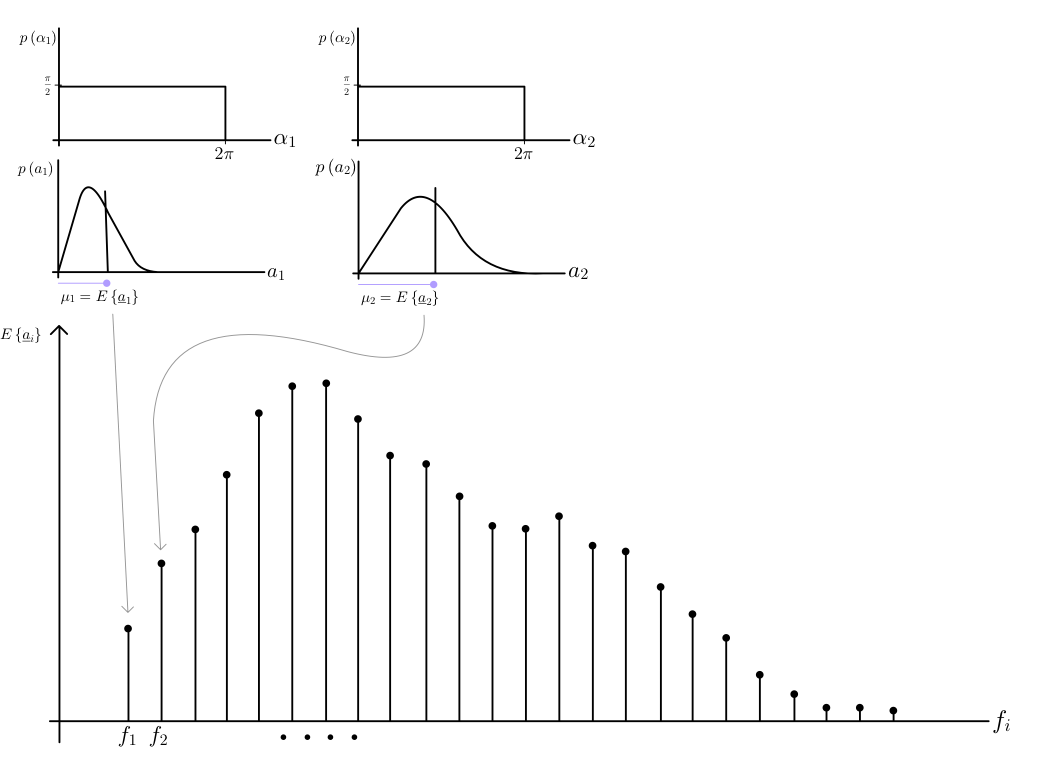
\includegraphics[width=.75\linewidth]{Figures/Theory/placeholder_randomModel.png}
    \caption{Visual explanation of the random phase/amplitude model. Every discrete frequency is represented by a uniform and Rayleigh distribution for the random phase and amplitude respectively. The top half of the figure depicts the random distributions at certain frequencies, and the bottom half depicts the amplitude spectrum as a function of frequency. Adapted from \cite{Holthuijsen2007}.}
    \label{fig:ap.randModel}
\end{figure}

\section{Energy Density Spectrum} \label{sec:sec:ap.oceanWaves.energySpectrum}
The energy density spectrum is more useful than the variance density spectrum as it shows the distribution of wave energy over various frequencies, where a narrower spectrum represents a more regular wave. The energy of a harmonic wave is given as the mean-square elevation times the gravitational acceleration, $g$, and the density of water, $\rho$. This gives the total energy as

\begin{equation} \label{eq:ap.waveSpectrum.totalEnergy}
   E_{total} = \rho g \overline{\underline{\eta}^{2}}
\end{equation}

Which allows the energy density spectrum to be obtained as

\begin{equation} \label{eq:ap.waveSpectrum.ESD}
   E_{energy}(f) = \rho g E_{variance}(f)
\end{equation}

